% TEX encoding = UTF-8 Unicode
% Compiled by XeLaTeX.

\documentclass[utf8, a4paper,11pt, onecolumn]{ctexart}
\usepackage{xeCJK}
\usepackage{setspace}				% set line space


\title{推荐系统的协同过滤算法实现与浅析}
%\author{}
%\date{\today}

\begin{document}
\begin{spacing}{1.3}

\maketitle
\tableofcontents
\newpage

\section{项目简介}

\subsection{摘要}

个性化推荐系统基于用户的历史兴趣和商品的特性,向用户推荐合适的信息或商品,其目前在互联网领域,尤其是电子商务、广告业务等方面,具有非常广泛的应用。推荐系统的进步,会更加迎合用户的需求,为产品赢得更好的口碑,创造更多的收益,形成一个良性的循环。因而,对推荐系统的研究在算法和实践中不断发展,不断进步。

本项目选择推荐系统为主题,基于(user, item, rating)数据集,预测没有评价的(user, item),以均方根误差RMSE为评价指标。

由于这门课是以算法为核心的课程,因而本项目更加注重算法的具体内容和细节。在项目中,所有核心代码均自己编写,没有调用任何外部算法模块。在报告中,也会主要以算法内容和实现细节为主。

在baseline的基础上,我实现了最基本的user-user和item-item协同过滤算法,以及基于baseline的协同过滤算法,验证了item-item相比user-user能获得更好的效果。同时,在基本的协同过滤算法上,加上了bias、TopK等优化,进一步提升了模型效果。此外,研究了TopK算法中,K的取值对模型效果的影响。最后,尝试融合了不同的算法并调参,获得了更好的融合模型。

在项目过程中,在计算统计量、相似度、预测等处,遇到了诸多算法细节问题,并进行了合适的处理。对于矩阵运算的代码,尽量进行了Vectorization,以提高速度。同时,自己重新组织了代码结构,分离了各个功能,使其具有更好的模块性,运行更加流水线化。

此外,对于数据集采用了k-fold 交叉验证,以交叉验证后的均值RMSE作为更稳定的评价指标。

\subsection{数据集}

原先,我采用的是NetflixPrize 数据集,NetflixPrize是关于电影评分的数据集。标准的NetflixPrize数据集包含了480189个user,和17770个item,以及总计约1亿的ratings。数据集中还包括了打分的时间,以及各部电影id对应的名称和年份。

对于协同过滤方法来说,该数据集产生的评分矩阵规模达$480189 \times 17770$,总元素约有80多亿,在该矩阵上的统计已经要耗时数十秒,对该矩阵进行更细粒度的计算则会更慢。

因而,我换用了一个规模更小的数据集MovieLens, 其数据方式与Netflix-Prize基本相同,它提供了不同规模的数据集,包括100K, 1M, 10M, 20M(均指Rating数)等多个规模的版本。

此外,相比于NetflixPrize,其提供了更多的信息,除了打分时间以外,包括用户的性别、年龄、职业、地区,以及电影的名称、发行时间、和丰富的标签(科幻、动作、文艺等)。

这些丰富的信息都是可以被推荐系统所利用的。如用户的年龄和职业可以被用来聚类,电影的标签可以用来做基于内容(content-based)的推荐,时间戳可以用来进行时序化的推荐(更新鲜的打分具有更高的权重),这些还可以同协同过滤算法相结合,从而达到提高预测速度和精度的目的。

此外,需要注意的是,数据集是经过过滤处理的,所有打分少于20个的用户均被过滤,因而,出现在数据集中的用户,每个用户至少对20部影片进行了打分。(而对于每部影片则不然,可能存在没有被打分的影片)

为了获得较快的执行速度,所有模型的结果均基于100K版本的MovieLens数据集。该数据集包括943 users, 1682 items, 100000 ratings.

\subsection{评价指标}
\label{评价指标}
评价指标选择均方根误差,其定义如下:

\[RMSE = \sqrt{\sum_{i = 1}^{N}(r_{xi} - \hat{r}_{xi})^{2}}\]
其中,$\hat{r}_{xi}$为用户$x$对项目$i$的预测打分,$r_{xi}$为用户$x$对项目$i$的实际打分。

在模型改进时,采用了交叉验证的方法,最后选择每组数据集的RMSE均值作为预测方法的最终RMSE值:(k为交叉验证的组数)

\[\overline{RMSE} = \frac{1}{k}\sum_{i=1}^{k}RMSE_{i}\]

\section{数据处理}

\subsection{平台和工具}

以OS X 10.11及Python 3.5为主要开发环境,使用Anaconda作为Python的科学发行版。

使用Jupyter Notebook作为生产力工具,可以进行方便的调试。

使用Numpy和Pandas作为矩阵运算和数据载入的工具。

使用Git作为版本管理的工具。

\subsection{数据格式与交叉验证}

通过Pandas的DataFrame读入数据。

原先,所有数据采用一组训练集和测试集,训练集和测试集规模比为$4:1$。即,训练集规模为80000,测试集规模为20000。

为提高指标稳定性,采用了K次交叉验证(K-fold Cross Validation)的方法。将数据切分为5个子样本,每次取4组训练,剩余一组用于测试,循环5次。在交叉意义下的评价指标可见\ref{评价指标}节。

数据每行格式为(user, item, rating, timestamp)。

读入数据后,在模型内部填充ratings矩阵,以user为行,item为列,形成$943 \times 1682$的矩阵。

测试时,所有测试函数以(user, item)对为输入参数,返回预测的rating。

\textit{\textbf{trick}: 数据集内数据id以1开始,内部变量索引以0开始,做适当调整即可。}
\section{模型详解与分析}
\label{模型详解}
\subsection{统计指标及baseline}

首先,对于输入数据进行一些统计分析。

针对矩阵的稀疏程度,只需做简单运算即可得到,打分矩阵的密度为 $5.04\%$。

对矩阵的每一行和每一列求平均值,得到了各个user和item的打分均值。需要注意的是,此处要过滤零值,只对非零值求平均,否则无意义。

\textit{\textbf{trick}: 过滤出非零值不需要每行(列)分别过滤,可以对每行(列)执行求和和非零值计数运算,直接相除。}

baseline是基于这些统计量的预测算法。其预测公式为

\[\hat{r}_{xi} = \mu + ub_{x} + ib_{i}\]

其中,$\mu$为总体均值,$ub_{x}$和$ib_{i}$分别是user x和item i的均值与总体均值的偏差。化简可得:

\[\hat{r}_{xi} = \overline{r_{user\ x}}+ \overline{r_{item\ i}} - \mu\]

此算法即为baseline的效果,其RMSE值为\textbf{0.9694}.

\textit{\textbf{trick}: numpy采用了float64类型存储浮点数,最好不要对其做任何近似操作,只需在最后的输出结果中采用近似表示即可。}

%(注: 实践证明,中间量近似可能会略微提高效果,但几乎可忽略,且不具有普遍性,可能是由于四舍五入后可能更接近整数打分导致)

\subsection{相似度矩阵与协同过滤}

协同过滤(Collaborative filtering)基于这样的思想:如果两个user对大多数item的打分相近,说明这两个user的相似度较高,或者若果两个item被大多数user打分相近,也说明这两个item的相似度较高。

基于相似度的来源,以上分别被称为user-user协同过滤和item-item协同过滤。

相似度采用Cosine距离测量,其公式为

\[sim(x,y) = \frac{r_x \cdot r_y}{\| r_x \| \| r_y\|}\]

该公式对行和列均有效。其对应的矩阵运算为:

\[Sim = \frac{R \cdot R^T}{\| R\cdot R^T \|}\]

\textit{\textbf{trick}: 为防止divide by zero错误,可以在计算时加上一个小偏差$\epsilon$。即,采用$R\cdot R^T + \epsilon$的方式进行实际计算。}

在得到user相似度和item相似度后,可以通过其相似度矩阵进行预测。

预测公式为用户对其它item打分和item之间相似度的加权平均(针对item-item协同过滤):

\[\hat{r}_{xi} = \frac{\sum_{j \in N(x)} s_{ij} \cdot r_{xj}}{\sum_{j \in N(x)} s_{ij}} \]

其中$N(x)$为user x打过分的数据。此处不能对所有数据求加权平均,因为其没有打过分的item,求平均值没有意义,反而会增加分母的值,导致预测严重偏差。

\textit{\textbf{trick}:该预测公式还需要一点补充,即冷启动问题,当该公式分母为0时,结果为NaN,此时可以采用baseline结果代替NaN.}

该方法基于item-item的交叉验证结果是\textbf{1.0149},竟然比baseline还高,而基于user-user的结果是\textbf{1.0174},同样超过了1。

\subsection{结合baseline的协同过滤}
所以,baseline的意义是重要的,只采用协同过滤,效果并没有那么明显。
将baseline和协同过滤结合起来,在baseline的基础上预测,更新公式为:

\[\hat{r}_{xi} = b_{xi}  + \frac{\sum_{j \in N(x)} s_{ij} \cdot (r_{xj} - b_{xj})}{\sum_{j \in N(x)} s_{ij}} \]

其中,$b_{xi}$为用户x, 项目i的baseline预测值,$N(x)$为用户x打过分的项目集合。同样可以采用向量化计算。

经过改进,基于baseline的item-item协同过滤算法可以将RMSE提高到\textbf{0.9362},相比于baseline有了很大的进步。

而基于baseline的user-user协同过滤也达到了\textbf{0.9548}.

可以得出,在实际应用中,的确item-item的算法表现更加好,大致是商品之间的相似程度,没有人的个性强。

\textit{\textbf{trick}:在进行到此处时,发现了一处细节优化,即由于最终打分必然是1-5的整数值,那么在预测时,若预测结果小于1,可以返回1为结果,若预测结果大于5,则返回5为结果。这个改进是微小但稳健的,其可以将item-item协同过滤RMSE由\textbf{0.9362}提高到\textbf{0.9360}}

\subsection{topK协同过滤与K值的选择}

在协同过滤的预测中,由于需要针对每个预测计算所有的历史数据,时间开销较大,且并不是所有打过分的项目,均属于和item较相似的范畴。因而,可以采取topK技巧,在所有打过分的item中,过滤出与该item相似度最高的K个item,只对这K个item进行加权平均。

\[\hat{r}_{xi} = b_{xi}  + \frac{\sum_{j \in N_k(x)} s_{ij} \cdot (r_{xj} - b_{xj})}{\sum_{j \in N_k(x)} s_{ij}} \]

\textit{\textbf{trick}: 如果用户打过的item数不足K,则直接使用所有打过的item。这也是基于某些用户可能只倾向于对其喜欢的商品评分。}

在运行时,在采用item-item协同过滤的情况下,选择K=10时,得到的RMSE为$1$选择K=40时,得到的RMSE为$1$.

可以发现,不同的K值,其效果非常不同。当K太小时,不能覆盖所有与其较相似的item, 而当K太大时,所选的item可能已经与其不再非常相似。

因而,此处不同的K值得到的RMSE应该呈现U型。

尝试调整K,对不同的K,得到的RMSE如表格\ref{k-table}.

\begin{table}
	\centering
	\begin{tabular}{| c | c | c | c | c |}
		\hline
		\textbf{K值} & item训练集 & item 测试集&user训练集 & user测试集 \\ 
		\hline
		5 & 0.5747 	& 0.9543 & 0.6101 &	0.9874 \\ 
		\hline
		10 & 0.6845 &	0.9278 & 0.7242 &	0.9573 \\
		\hline
		15 & 0.7322 &	0.9223 & 0.7699 &	0.9489 \\
		\hline
		18 & 0.7500 &	0.9215 &	0.7866 &	0.9468 \\
		\hline
		20 & 0.7596 &	0.9213 & 0.7951 &	0.9458 \\
		\hline
		25 & 0.7774 &	0.9217 &	0.8113 &	0.9449 \\ 
		\hline
		30 & 0.7902 &	0.9225 &	0.8225 &	0.9445 \\
		\hline
		40 &0.8073 &	0.9242 &	0.8373 &	0.9447 \\
		\hline
		50 & 0.8182 &	0.9258 &	0.8465 &	0.9453 \\
		\hline
		100 & 0.8422 & 0.9314 &	0.8660 &	0.9491 \\
		\hline
		200 & 0.8546 &	0.9345 &	0.8747 &	0.9526 \\
		\hline 
	\end{tabular}
	\caption{不同K值下的RMSE}
	\label{k-table}
\end{table}

可以看出,随着K的增大,训练集上的RMSE逐渐增大,而不是一般意义上的逐渐变小,其原因主要是,训练数据融入了均值和相似度,在预测时不可避免地利用到了原先的信息。

值得注意的是,在user-user协同过滤算法上,测试集的RMSE中间较为平缓,因而可以发现对于user而言,需要更多的相似用户去衡量这个用户的属性,也即,user之间的差异比item之间的更大一些。

可以画出对应的RMSE曲线,如图\ref{k-figure}。

\begin{figure}
	\centering
	\includegraphics[width=0.8\linewidth]{k-figure.png}
	\caption{不同K值下的RMSE变化图}
	\label{k-figure}
\end{figure}

测试集上的确呈现出非典型的U型,U型的低谷即为对应的最优K值。事实上,采用更多的数据,边缘数据由于其权重的减少,对最终预测值的影响也减小,类似于经济学中的边际效应递减规律。

另外,值得说明的是,显而易见,不同规模的输入,应该要有不同大小的K值相匹配。更大规模的数据,应该需要更大规模的K值。

\textit{\textbf{trick}:在这里,我采用的方式是直接设定一个K值集合,因而对于不同规模不具有很好的适应性。更好的方式则是通过学习,例如采用梯度下降,去逼近一个较优的K值。}

对于该数据集而言,当采用item-item协同过滤时,K=20为宜,RMSE为\textbf{0.9213},当采用user-user协同过滤时,K=30为宜,RMSE为\textbf{0.9445}.

\subsection{归一化的相似度矩阵}

在相似矩阵中,除了采用Cosine距离外,还可以有其它的相似度定义。

例如采用Pearson相关系数,其在算Cosine距离前,首先将同一行(列)的元素减去其平均值,以抹去各人打分标准不同所带来的权重差异,在这个意义下定义了新的相似度矩阵。

\[sim(x,y) = \frac{\sum (r_{xs}-\overline{r_{x}}) \cdot (r_{ys}-\overline{r_{y}})} {\sqrt{\sum (r_{xs}-\overline{r_{x}})^2} \sqrt{\sum (r_{ys}-\overline{r_{y}})^2}}\]

此即为归一化的相似度矩阵定义。同样,采用向量化方式将加快该矩阵的计算。

而同时用于预测的函数,可以保持不变,仅将其中采用的相似度矩阵换成归一化后的相似度矩阵即可。

然而,在topK item-item协同过滤的基础上,将原先的相似度矩阵替换为归一化后的相似度矩阵,其RMSE反而从\textbf{0.9213}提高到\textbf{0.9253}。

至于为什么会出现RMSE反而提高的情况,经与老师讨论及相关查阅后,发现这与数据集本身的一些性质有关,对于某些打分很少的item,做归一化之后,其反而抹去了这些item原来就已经很少的信息。例如一部小众的影片,三四个口味相符的受众同时打出了5分的高分,则归一化之后,一下子抹去了这部电影的高分信息,反而产生了信息的损失。

在这种情况下,忽然想到,那对于user-user协同过滤,由于该数据集中,每个用户至少打过20个评分,那么这样的弊端应该会被尽量避免。于是,尝试对user-user协同过滤采用归一化后的相似度矩阵,然而效果同样不尽人意。


\subsection{模型融合与融合参数}

此时,协同过滤算法的各种优化价值似乎已经被压榨完。突然灵光一现,想到NetflixPrize最后的获奖算法,多层次多尺度地融合了三百多个模型。所以,是否可以借鉴这样的思路,尝试一下模型融合在这种情况下,会产生怎样的效果?

在以上的模型中,具有本质区别的只有两种,item-item协同过滤和user-user协同过滤。于是,尝试将这两者相融合。其中,K值分别选取20和30,也即其各自的最优值。

\[\hat{r}_{xi} = \frac{\hat{r_1}_{xi} + \hat{r_2}_{xi}}{2}\]

果真得到了更好的效果,item-item协同过滤的RMSE为\textbf{0.9213}, user-user协同过滤的RMSE为\textbf{0.9445},而将两者的预测结果取均值,优化效果非常明显,RMSE降低到了\textbf{0.9176}.

进一步,由于item-item协同过滤的效果更好,所以我认为,应该在模型融合时对其采用更大的权重,于是,定义预测函数为:

\[\hat{r}_{xi} = 0.6 * \hat{r_1}_{xi} + 0.4 * \hat{r_2}_{xi}\]

得到了更好的RMSE值,为\textbf{0.9159}. 可以看出,模型融合的意义很大。

类似在topK方法中的思路,可以将公式改进为线性融合函数:

\[\hat{r}_{xi} = \alpha * \hat{r_1}_{xi} + (1-\alpha) * \hat{r_2}_{xi}\]

其中,$\alpha \in [0, 1]$,在端点处即分别为两个模型,而系数$\alpha$则表示了融合程度,也即在融合模型中item-item协同过滤的权重。

通过调参,调整$\alpha$的值,可以获得最佳的融合效果。

在不同的$\alpha$值下测量RMSE,得到表\ref{alpha-table}.

\begin{table}[h]
	\centering
	\begin{tabular}{|c|c|c|}
		\hline
		\textbf{$\alpha$} & 训练集RMSE & 测试集RMSE \\
		\hline
		0.00 & 0.8225 & 0.9445 \\
		\hline
		0.10 & 0.8108 & 0.9368 \\
		\hline
		0.30 & 0.7907 & 0.9248 \\
		\hline
		0.50 & 0.7754 & 0.9176 \\
		\hline
		0.60 & 0.7696 & 0.9159 \\
		\hline
		0.65 & 0.7672 & 0.9155 \\
		\hline
		0.70 & 0.7651 & 0.9154 \\
		\hline
		0.75 & 0.7634 & 0.9156 \\
		\hline
		0.80 & 0.7620 & 0.9161 \\
		\hline
		0.90 & 0.7601 & 0.9181 \\
		\hline
		1.00 & 0.7596 & 0.9213 \\
		\hline
	\end{tabular}
	\caption{不同融合参数$\alpha$下的RMSE}
	\label{alpha-table}
\end{table}

同样,画出不同$\alpha$下,融合模型的RMSE变化趋势(图\ref{alpha-figure})。

\begin{figure}[ht]
	\centering
	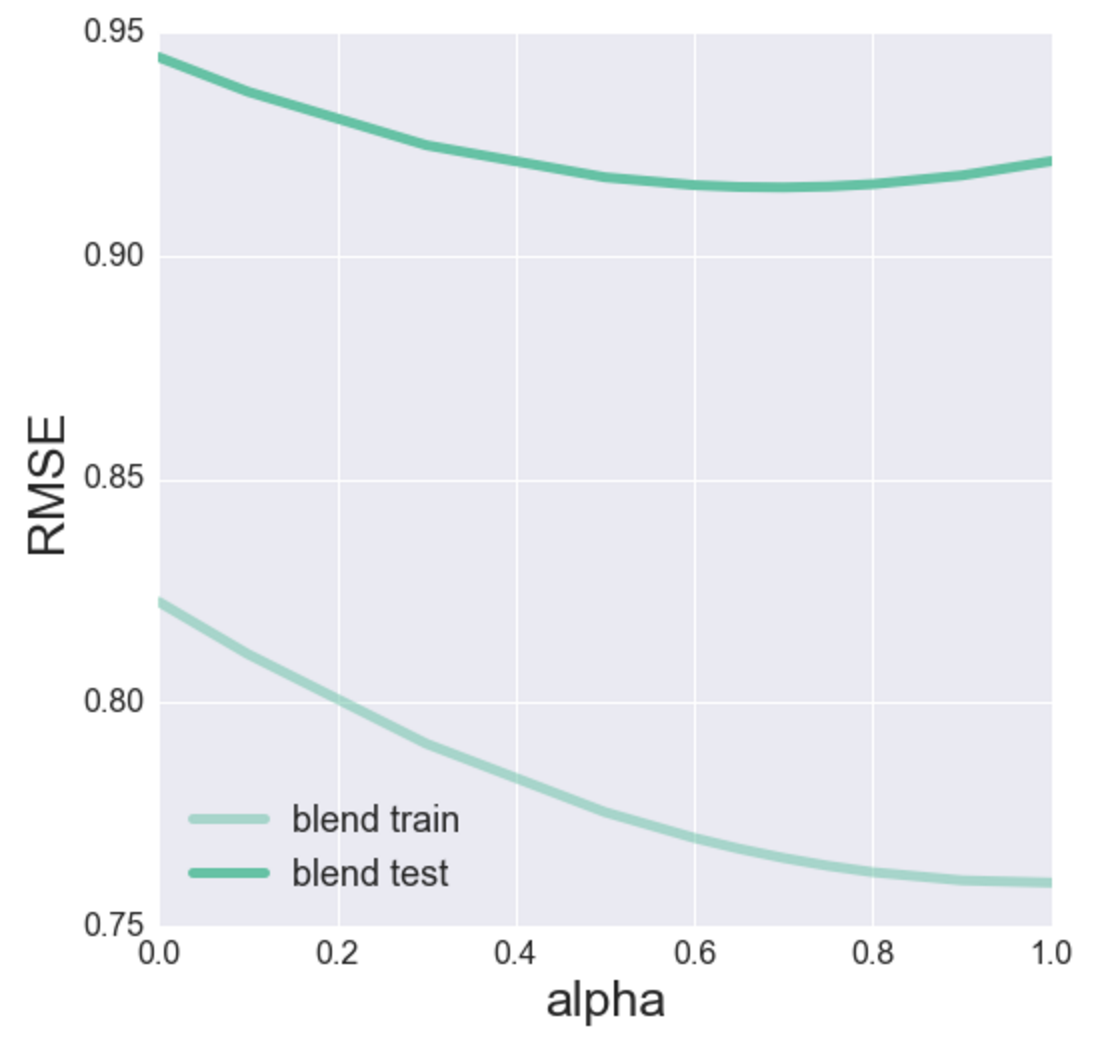
\includegraphics[width=0.8\linewidth]{alpha-figure.png}
	\caption{不同$\alpha$值下的RMSE变化图}
	\label{alpha-figure}
\end{figure}

最终,选取$\alpha = 0.70$,得到了\textbf{0.9154}的RMSE。

此外,还可以考虑一些非线性的模型融合方式。

\section{模型结果}

在模型详解(第\ref{模型详解} 节)中,详述了各个模型的定义、公式、相关分析,以及各种trick。

其最终的RMSE比较为表格\ref{RMSE-table},需要注意的是,这其中很多方法都是建立在前者的方法上,叠加了前面的方法,一点点尝试改进。

\begin{table}[h]
	\centering
	\begin{tabular}{|c|c|}
		\hline
		\textbf{方法} & \textbf{RMSE} \\
		\hline
		baseline &   0.9694 \\
		\hline
		itemCF &  1.0149 \\
		\hline
		userCF & 1.0174 \\
		\hline
		itemCF+baseline &  0.9362 \\
		\hline
		userCF+baseline & 0.9548 \\
		\hline
		itemCF+bias & 0.9360 \\
		\hline
		topkCF(item, k=20) & 0.9213 \\
		\hline
		topkCF(user, k=30) &0.9445 \\
		\hline
		normCF(item, k=20) &0.9253 \\
		\hline
		blendCF($\alpha$=0.7) & 0.9154 \\		
		\hline
	\end{tabular}
	\caption{不同方法的RMSE比较}
	\label{RMSE-table}
\end{table}

最终,在不断进行各类优化后,融合了两个topkCF模型的blendCF模型取得了\textbf{0.9154}的RMSE值。

\section{总结}

在这个项目中,我不断尝试新的思路,改进已有的算法,去获得更好的预测效果。通过这一过程,我对推荐系统的协同过滤算法,有了更加深刻的理解。

统计量是非常简单却又及其重要的一个指标,如果不基于baseline,算法好像失去了一个有力的支点,其效果可能不尽人意。

最基本的协同过滤算法,采用相似度的衡量方式进行预测。其效果和维度本身的差异性有关,但总是能带来较为显著的效果提升。

topK算法则更进一步,大大提升了模型效果。其中,关于K值的选择,也非常值得探讨。在现实场景中,这个参数可以通过学习获得。

原本以为归一化的相似度矩阵,会对模型带来深刻改进,但至于为什么RMSE反而提高了,目前还不太理解。这也是以后可以进一步研究的地方。

最后,模型的线性融合,是一个非常易于实现,且能够提升预测效果的方法。模型的融合在各种现实应用场景中也非常地普遍,其融合的各种技巧,还可以继续探究。

此外,算法中,关于divide by zero等处理细节,以及 Vectorization等技巧,可以达到避免潜在风险、提升算法效率的作用。

算法实践过程中,也遇到了不少的问题和困惑,请教了老师,同时阅读了历史上一些相关领域的经典论文\cite{breese1998empirical}\cite{sarwar2001item},理解了这之中不同算法细节的优缺点和应用场景。

其实,这个数据集上还可以做更多的工作,例如利用电影的标签,进行基于内容的推荐。而在应用到现实场景中时,电影的发布时间也会成为一个推荐的因素,人们更倾向于观看更新的影片。

总而言之,通过这个动手项目,第一次采用了Numpy, Pandas等科学计算库,锻炼了手写算法的能力,加深了对协同过滤的理解,从中学到了很多。


%\renewcommand\refname{参考文献}
\bibliographystyle{plain}
\bibliography{Report}

\end{spacing}
\end{document}
